\chapter[Bidding]{Bidding Method}
\label{AppendixA}

\section{Incorporating growth and discounting}
%We need a time period T for calculations. For use in any calculation, 
The rates $\delta,\ t,\ r_i$ depend on the period, $T$. For example, with a current price of $P_0$, a price-growth rate of $\dot p$ per year, and a 5 year mortgage period, the expected price in $T$ years is:

% WHY DOES THIS DEPEND ON MORTGAGE? - do without 5 years first.

\[P^e_T=P_0(1+\dot p)^T\]

% the current price is , 
The T-year growth rate is $(1+\dot p)^T$. If, for example, $\dot p= 0.1$, or 10 \%, The growth  over a 5-year mortgage term or capital gain, would be 0.61051 or 60\% of the original price.

Similarly, if we want the compounded interest rate for person $i$ the term T,
\[Rate_i^T=(1+r_i)^T\]
This is the value we use in equation~\ref{EqBidPrice}.


If person $i$  discounts at $discr_i$, the present value of  a receipt at time $T$ is calculated by using the \textbf{discount factor} $\delta_i^T$.

\[\delta_i^T= \left( \frac{1}{1+discr_i} \right)^T \]
%\[\delta_i^T= \sum_{\tau=0}^{\tau=T}\left( \frac{1}{1+discr_i} \right)^\tau \]
 
These can be combined into a function %\deltathat  gives  a single discounting factor  for a value  like future price that is both growing and being discounted over several (T) periods:
\[ PDV(P^e_T)=P_0\left( \frac{1+\dot p}{1+discr} \right)^T \]
This PDV function specifically combines any expected rent increase, the individual's discount rate and the mortgage term into a single operation. 




\subsection{Mortgage availability}

For home loans, many personal finance experts recommend total housing costs account for less than 28\% of your \textbf{gross} household income, This gives us an \textbf{income-based  mortgage maximum} of \[M^{max}_Yi = \frac{0.28*(\omega+w)}{r_i}\] It is the maximum the bank will let you pay.

We assume $r_i$ is based on the individual's assets, on relative wealth. Where is it calculated for the householder or the bank?

We get a \textbf{price-based mortgage maximum} \[M^{max}_P = 0.8P_0\] where $P_0$ is the actual sale price. This is based on the maximum amount of risk that the bank is willing to take on. ( $P_0$  will not always be the same as the asking price or the warranted price.) 

\subsection{Investment decision and bid price}
The value of a property purchase over the course of a mortgage term is the capital gain minus the financing cost plus the net rental income, $\mathcal{R}$:
\begin{align}
V  	&= Net\ Capital\ Gain && + \mathcal{R}\\
    &=  Capital\ gain - Interest\ due  +	    &   Rent  - Operating\ cost - Taxes \\
    &= \delta(P_T- (1+r)M)             	& + R  	-C  - T\label{B2} \\
    &= \ \delta((1+\dot p)  P_0- (1+r)mP_0)  & + \rho P_0  - \kappa P_0 - \sigma P_0 \\
    &= (\delta((1+\dot p)  - (1+r)m)        & + \rho - \kappa  - \sigma) P_0 
\end{align}

This can be expressed in terms of the rate of return on the down payment
\begin{eqnarray}
v &=&( \delta((1+\dot p)  - (1+r)m) \    + \rho  - \kappa - \sigma) \frac{P_0}{D}   \nonumber \\
  &=& (\delta((1+\dot p)  - (1+r)m) \    + \rho  - \kappa - \sigma) \frac{P_0}{P_0-mP_0}   \nonumber \\
  &=&\frac{ \delta(1+\dot p  - (1+r)m) \ + \rho  - \kappa - \sigma} {1-m} \label{Eqn:DecisionRule}
\end{eqnarray}

RULE: invest if $v$ is greater than  the  target interest rate $r_{target}$. The formula is developed below.


\section{Market behaviour}
Equation~\ref{Eqn:DecisionRule2} provides a behavioural criterion for investors: invest if $v \geq r_{target}$. The equation lets us a  maximum price that satisfies this criterion, which we define as the ``bid price'', $P^{max}_{bid}$. The bid price is used in the price determination process in our model. 

The  price at the end of the term,  $P_T$, is a predicted value  for the investor \textit{ex-ante}, so we replace $P_T$ in Equation~\ref{Eqn:V} with $(1+\dot p)P_{bid}$. Then we replace $\dot p$ with $L(P)$ representing some estimated function of the lagged values of $P$ and any  other relevant data. It is  convenient to also replace $(\rho -\kappa - \sigma)P_0$ with $\mathcal{R}_N$ (net rent). he result is 

\begin{eqnarray}
v %&=& \delta(P_T- (1+r)M) \qquad \qquad \qquad 	 + \mathcal{R}_N \nonumber\\
% &=&\delta\left( (1+\dot p)P_{bid} - (1+r)mP_{bid} \right)  + \mathcal{R}_N  \nonumber\\
  &=&\delta\left( (1+L(p)) - (1+r)m \right) P_{bid} + \mathcal{R}_N  \nonumber
\end{eqnarray}

The rule is, ``Bid if the RHS is larger than the target rate of return, $r_{target}$, and do not bid if it is smaller.''  The maximum bid  is the bid that makes the two sides equal. 

\begin{eqnarray}
%r_{target}&=& \delta\left( (1+L(p)) - (1+r)m \right) P^{max}_{bid} + \mathcal{R}_N  \nonumber\\
   P^{max}_{bid} &=&\frac{r_{target} - \mathcal{R}_N}{\delta\left((1+L(p)) - (1+r)m \right)} \label{EqBidPrice} 
\end{eqnarray}
In practice, potential investors will make an  initial  bid that is lower than this value and subsequent bargaining will settle of a price between the initial bid and the seller's asking price.


\section{Finding bid price}
We start with Equation~\ref{B2}. for convenience, replace $\rho -\kappa - \sigma $ with $\mathcal{R}_N$ (net Rent). 

Replace $P_T$ with $(1+\dot p)P_{bid}$.

Then replace   $\dot p$ with $L(p)$ representing some (estimated function ($\tilde{\dot p}$)) of the lagged values of $P$ that incorporates other data. 

\begin{eqnarray}
v&=& \delta(P_T- (1+r)M) \qquad \qquad \qquad 	 + \mathcal{R}_N \nonumber\\
 &=&\delta\left( (1+\dot p)P_{bid} - (1+r)mP_{bid} \right)  + \mathcal{R}_N  \nonumber\\
  &=&\delta\left( (1+L(p)) - (1+r)m \right) P_{bid} + \mathcal{R}_N  \nonumber
\end{eqnarray}


So I want to use this relationship to find the maximum bid price for the bank. The rule is, ``Bid if the RHS is larger than the target rate of return, $r_{target}$, and do not bid if it is smaller.''  The maximum bid  is the bid that makes the two sides equal. 

{\color{red}
\begin{eqnarray}
r_{target}&=& \delta\left( (1+L(p)) - (1+r)m \right) P^{max}_{bid} + \mathcal{R}_N  \nonumber\\
   P^{max}_{bid} &=&\frac{r_{target}-\mathcal{R}_N}{\delta\left( (1+L(p)) - (1+r)m \right)} \label{EqBidPrice} 
\end{eqnarray}}
(What makes. this work is that I do not use an identity to get
$\dot p$, which made the system of equations singular.)
\newpage

\subsection{On Bidding}

In the market, the initial bid should be smaller than the bid price calculated, which is a maximum that can earn the target rate of return, The bank will definitely go this high. 

If there is a  max bid among competing buyers, the second highest max bid should be the sale price, but the bidder with the highest max bid wins the property. This makes sense because in a bidding war the final bid only has to be a very small amount higher than that of the last competitor left.
That is the highest price that a seller can get.

It might be simplest to treat every seller as a bidder. All bid above here own are considered. The one chose ins the second highest. This  seems realistic enough and is very simple to implement. It should producer a path that is indistinguihable form any more com[plex apporach] 

Will peersons retireing who would lerave the city invest in an urban rental?

This should 


Bargaining between buyers and sellers differs. Buyers bid low and sellers ask high.  {\color{red}We need to calculate a minimum selling price for the seller}.



% But what is $D$? Does the bank have unlimited funds? Isn't D just a fraction of P?  If so it cancels out

% r is the prime rate- that the bank pays? 

\section{Relating the equations to the code}
Taking the expression for $P^{max}_{bid}$, we now discuss each of the terms and how they are implemented in the code. The following subsections are numbered consistent with this layout "
\[\frac{B4.1-B4.2}{B4.3\left( (1+B4.4 - (1+B4.5)B4.6\right)}\]

\subsection{Computing the target interest rate, $r_{target}$}
prime rate plus a margin required by the bank.  Question: do non-bank actors have such a term?

\textbf{CODE:}   self.get-target-interest-rate(buyer).


\subsection{Computing net rent}
Net rent is
$\mathcal{R}_N = (1-\kappa_j - \sigma_j) (\omega-tau*d_j)$


The tax ratio is an important number - it is the share of rents that the municipality takes for services and infrastructure. I estimate it to be about 30\% so $t=0.3$.


In reality, $\kappa$ this varies for every property based on maintenance requirements, historic rents, tenant rights, and variations in assessed values. This will matter for the buyer. If it varies may be useful as a quality indicator.

Values for $\kappa$ and $\sigma$ must be adjusted to take into account the length of the period or net rents have to be summed over the period


If we want to know the  present value  of the \textbf{net rent}, $\mathcal{R}_N$, we collect over the period  $\mathcal{R}_N^T$, we \textbf{add up} the rents each year. We  assume the rents are rising and  collected at the end of the year and the first is $\mathcal{R}_N0$.
\[\mathcal{R}_Nj^T= (\omega-tau*d_j)\sum_{\tau=0}^{\tau=T-1} \frac{(1+\dot{rent})^{\tau}} {(1+r_{discr_i})^{\tau+1}} \]

% \[\mathcal{R}_Nj^T= (\omega-tau*d_j)\sum_{\tau=0}^{\tau=T-1}\left[\frac{1+\dot{rent}}{1+r_{discr_i}}\right]^\tau \]
where $\dot{rent}$ is an expected rate of change of rents - possibly zero for now, and $discr_i$ is the individual's discount rate.



\textbf{CODE:}  

\subsection{Computing the discount factor for T, $\delta$}
The discount factor $\delta_i$ captures the cost of waiting T periods to sell the property. The usual; way to treat it, which we use here, is to assume that $i$ has an interest rate $r_i$ and has been investing efficiently. This means that  the individual has a discount factor for future returns base on the year-over-year rate of return. 

\[\delta_i=\left[\frac{1}{1+r_i}\right]^T\]

\textbf{CODE:}  
\subsection{Computing the approximation function for price forecast $L(p)$}
$p$ is all the price data plus any exogenous information (EG Policy knowledge?). $L(p)$ is an estimation function that produces a `common knowledge' value for the rate of price increase. Later you can add idiosyncratic extra knowledge or extra ignorance.

\textbf{CODE:}  Kirsten has to come up with a data aggregator 



\subsection{Computing the bank's interest rate, $r$}

I think this is just the bank rate set by the Bank of Canada. Exogenous. Just define it.

\textbf{CODE:}  

\subsection{Computing the borrowing ratio, $m_i$}
The borrowing ratio is just the fraction of the price that the bank will lend. It may depend on the individual. It is likely to be higher for the ban and for rich people because the bank thinks rich people are more secure risks. they may have other assets that could be attached in the case of default.


I have suggested The cost of capital is known to differ for rich and poor. We need a function that captures this relationship so we need to define individual wealth:
\[W_i= P_i -M_i  +S_i\]
where 

\begin{tabular}{ll}
$P_i$ & value of owned home\\
$M_i$ & Mortgage on owned home\\
$S_i$ & personal savings = $age*d*W$\\
\end{tabular}

Here we should use the same logic as we use about the interest rate charged, $r_i$ - it should depend on the person's assets compared to others. The bank, as a person has lots of assets, so $m_i$ is close to one, say 0.9. For the average wealth holder, $m_i$ should be around - let's say, 0.8. 

We  tie the borrowing ratio, $m_i$,  for agent $i$, to individual wealth. Figure~\ref{Fig:Borrowingratio} illustrates a mortgage availability  model that is written 
 \[ m_i = 0.1(9-\left(\frac{W_i}{\bar W}\right)^{0.5}/2 )\]
Where $\bar{W}$ is mean wealth and $W_i$ is individual wealth. 




\textbf{CODE:}  

\begin{figure}
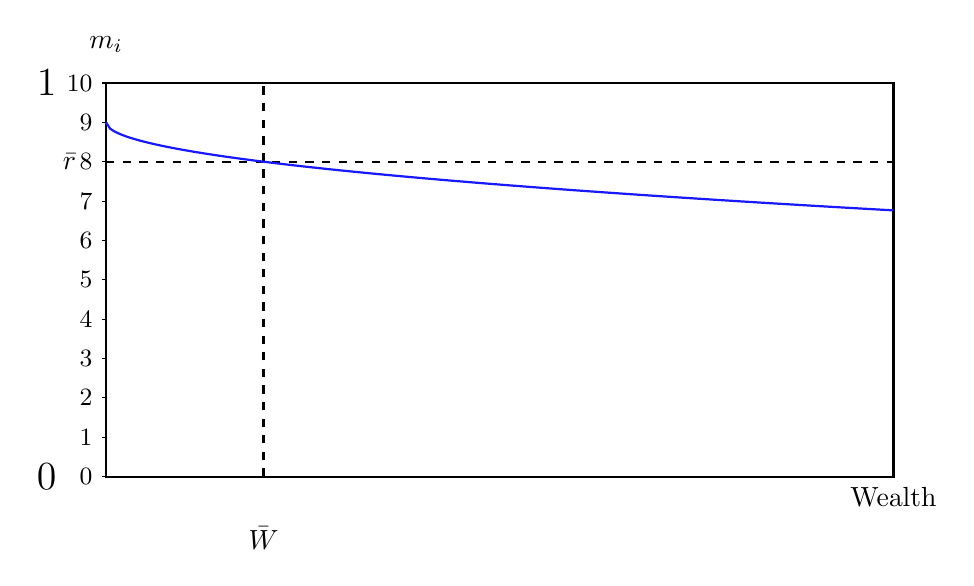
\begin{tikzpicture}[scale=.5]

%\def\bndmax{5}        %https://tex.stackexchange.com/questions/68462/filling-a-complex-region-with-tikz
%\def\bndmin{0.2}
\def\Y{10}  % height of y axis pecent
\def\W{20}  % length  of x axis
\def\Wbar{4} % meam wealth
\def\rbar{8}% this is the prime rate

% %Equation   \[ r_i = (A + .5 \frac{\bar{W}}{W_i})\omega\]
   % \def\Wmin{.63}  %This sets the lower limit fo the 
    \def\Wmin{(\B*\Wbar)/(\Y/\rbar-\A)} %function to keep in in bounds
	
 \tikzset{func/.style={thick,color=blue!90}}	

 \draw [thick](\W,\Y)-- (0,\Y)node[left=.5cm]{\Large$1$}node[above=.25cm]{$m_i$} -- (0,0)node[left=.5cm]{\Large$0$}--(\W,0)node[below]{Wealth}--cycle;  	% Axes
 \draw [dashed, thick] (0,\rbar)node[left=.25cm]{$\bar r$} -- (\W,\rbar);  	% Axes
\draw [thick,dashed] ( \Wbar,0)node[below=.5cm]{$\bar{W}$} -- (\Wbar,\Y);  	% Axes

\foreach \yi in {0,...,\Y} \draw (0,\yi)--(-.1,\yi)node[left]{\small$\yi$};
%\foreach \yi in {0,2,4,6,8,10} \draw (0,\yi)--(-.1,\yi));
%node[left]{\small$\yi$};
%\foreach \yi in {0,2,4,6,8,10}node at (-.1,yi) {{10*yi}} ;
\draw[func,domain=0:\W] plot [samples=200] (\x,(9-\x^.5/2);

 \end{tikzpicture}
\caption{Individual borrowing cost as a function of wealth}
 \label{Fig:Borrowingratio}
\end{figure}



\subsection{Computing the individual borrowing rate, $r_i$}
In our model, we  tie the individual cost of capital,  $r_i$ for agent $i$, to a prime rate, $\bar r$ or the bank's target rate, $r_{target}$, prime plus 1\%, say. and to individual wealth. Figure~\ref{Fig:Borrowingrate} illustrates a couple of possible  cost-of-borrowing models roughly consistent  with the stylized facts about lenders. 
 \[ r_i = (A + B \frac{\bar{W}}{W_i})\bar r\]
Where $\Bar{W}$ is mean wealth and $W_i$ is individual wealth. 


Here is a function for  the individual interest rate

\begin{figure}
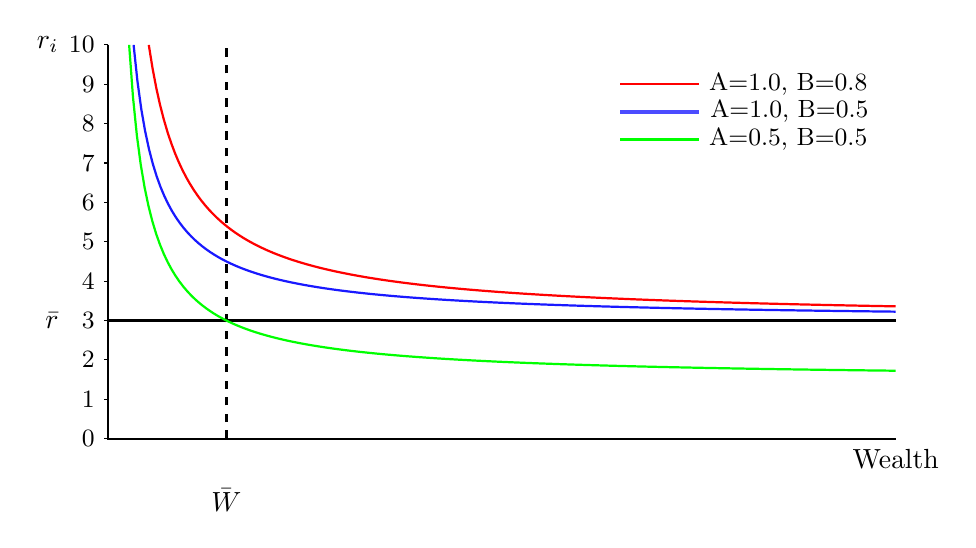
\begin{tikzpicture}[scale=.5]
%\def\bndmax{5}        %https://tex.stackexchange.com/questions/68462/filling-a-complex-region-with-tikz
%\def\bndmin{0.2}
\def \Y {10}  % height of y axis pecent
\def \W {20}  % length  of x axis
\def \Wbar {3} % meam wealth
\def \rbar {3}% this is the prime rate 

%Equation   \[ r_i = (A + .5 \frac{\bar{W}}{W_i})\omega\]
\def \Wmin{.63}  %This sets the lower limit fo the 
\def \Wmin{(\B*\Wbar)/(\Y/\rbar-\A)} %function to keep in in bounds
\tikzset{func/.style={thick}}	
	% Axes
\draw [thick] (0,\Y)node[left=.5cm]{$r_i$} -- (0,0)--(\W,0)node[below]{Wealth};  
\foreach \yi in {0,...,\Y} \draw (0,\yi)--(-.1,\yi)node[left]{\small$\yi$};
\draw [thick] (0,\rbar)node[left=.5cm]{$\bar r$} -- (\W,\rbar);  	% Axes
\draw [thick,dashed] ( \Wbar,0)node[below=.5cm]{$\bar{W}$} -- (\Wbar,\Y);  	% 

\def \A {1.0}  \def \B {0.5} %BLUE
\draw[func,domain=\Wmin:\W, color=blue!90] plot [samples=200] (\x,{(\A+\B*\Wbar/\x)*\rbar});
\draw [ultra thick, color=blue!70 ](13, 8.3)--(15,8.3)node [right, black] {\small A=\A,\ B=\B};

\def \A {0.5} 
\def \B {0.5} %GREEN
\draw[func,domain=\Wmin:\W, color=green] plot [samples=200] (\x,{(\A+\B*\Wbar/\x)*\rbar});
\draw [thick,  color=green](13, 7.6)--(15,7.6)node [right, black] {\small A=\A, B=\B};

\def \A {1.0}  \def \B {0.8} % RED
\draw[func,domain=\Wmin:\W, red] plot [samples=200] (\x,{(\A+\B*\Wbar/\x)*\rbar});
\draw [thick,  color=red](13, 9)--(15,9)node [right, black] {\small A=\A,\ B=\B};
% % KEY


 \end{tikzpicture}
\caption{Individual borrowing cost as a function of wealth}
\label{Fig:Borrowingrate}
\end{figure}


TESTING another function
\[ r_i  = (\bar r- A + B *\frac{\bar W}{W_i-C}) \]  
where A= y-shift, B= scale, and C= x-shift for the curve.

\begin{figure}
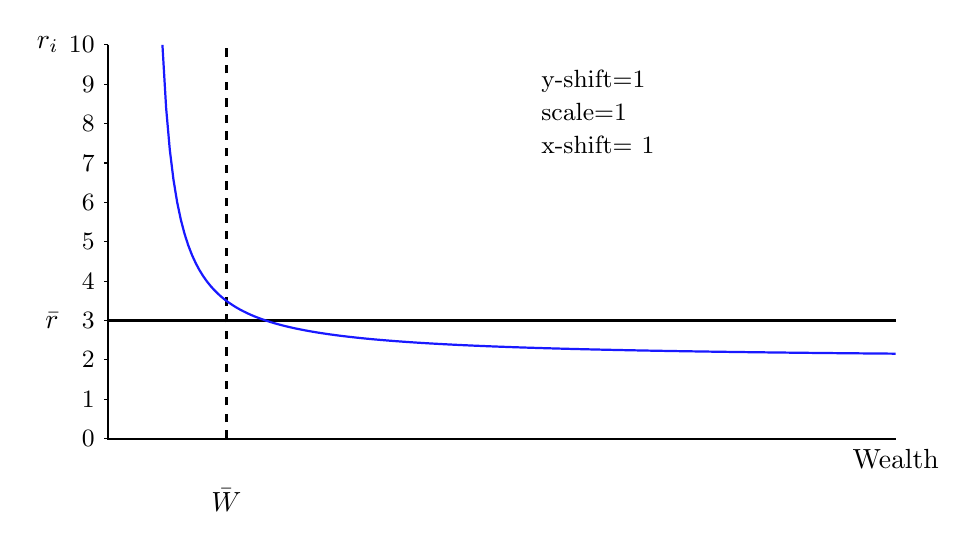
\begin{tikzpicture}[scale=.5]
%\def\bndmax{5}        %https://tex.stackexchange.com/questions/68462/filling-a-complex-region-with-tikz
%\def\bndmin{0.2}
\def \Y {10}  % height of y axis pecent
\def \W {20}  % length  of x axis
\def \Wbar {3} % meam wealth
\def \rbar {3}% this is the prime rate 

%\def \Wmin{(\B*\Wbar)/(\Y/\rbar-\A)} %function to keep in in bounds
\tikzset{func/.style={thick}}	
	% Axes
\draw [thick] (0,\Y)node[left=.5cm]{$r_i$} -- (0,0)--(\W,0)node[below]{Wealth};  
\foreach \yi in {0,...,\Y} \draw (0,\yi)--(-.1,\yi)node[left]{\small$\yi$};
\draw [thick] (0,\rbar)node[left=.5cm]{$\bar r$} -- (\W,\rbar);  	% Axes
\draw [thick,dashed] ( \Wbar,0)node[below=.5cm]{$\bar{W}$} -- (\Wbar,\Y);  	% 

\def \A {1} %vertical shift aroung \rbar, the prime rate
 \def \B {1}  % Scales the exponential curveBLUE
 \def \C {1}  %right shift  
% \def \Wmin {.4+\B}  %This sets the lower limit fo the 
\def \Wmin {(\B*\Wbar)/(\Y-\rbar+\A) +\C} %function to keep in in bounds

\draw[func,domain=\Wmin:\W, color=blue!90] plot [samples=200] (\x,{\rbar-\A+\B*\Wbar/(\x-\C))});
\node  [align=left, text width =2cm ] at (13, 8.3) {\small y-shift=\A \newline scale=\B \newline x-shift= \C};

 \end{tikzpicture}
\caption{Individual borrowing cost as a function of wealth II}
\label{Fig:Borrowingrate}
\end{figure}

\textbf{CODE:}  




\chapter[Parameters]{Parameter Values}
\label{AppendixB}

\section{Notation Table}

% \documentclass{standalone}
% \usepackage[dvipsnames]{xcolor}       \usepackage{calc}     
% \usepackage{tikz}
% \usetikzlibrary{shadings, shadows, shapes, arrows, calc, positioning, shapes.geometric}
% \usepackage{pgfplots}
% \pgfplotsset{compat=1.16}
% \usepackage{mathtools,amssymb}

% \begin{document} 
% \section{Notation for Urban and Production Sectors}

% $t$     & Time \\ 

t is time
TODO - uncomment the commented out ones with fraction- unidentified control sequence

delta is density ** - - infitesmal density increase as the city moves out. [[adjustment speed for wage N]] imagine a density function over the city. 
using the geometry for the derivative of that with respect - how does it change if you increase the amount under the integral, wehre does it go..  - in cont terms.  

N is population, n
d is diameter %(https://www.overleaf.com/project/606a6b286ae1c9f203fadab5 ). \\
omega is wage premium - which gives  the parented population
tau is linear transport cost per unit distance


\newpage
\begin{longtable}{lp{10cm}}
\caption{Notation}                \\

\hline           &  \textbf{Productivity} \\ \hline
$K$              &  Capital               \\ 
$L$              &  Labour                \\
$N$              &  Population, which equals labour, $L$ \\ 
% $n_i$  &  Number of workers employed by firm $i$ \\
% n=\sum_i n_i$  &  Number of workers, the urban population in the model \\
% $\#f=\frac{n}{n_i}$&number of identical firms \\ %not used
% $f$  &  Number of firms =1 \\
% $n =f n_i$  &  Aggregate labour \\
% $\Lambda(n)$    &  Labour-augmenting agglomeration effect \\
% $n^\gamma$ & The labour-augmenting agglomeration effect,  modelled as an exponential function of the number of people \\
% $\Lambda(n)n_i$ &  Effective labour for firm $i$ \\
% $\Lambda'=\die{\Lambda(n)}{n} $ & Derivative of the labour-augmenting agglomeration effect\\
$\alpha$         &  Elasticity of output with respect to capital          \\
$\beta$          &  Elasticity of output with respect to effective labour \\
$\gamma$         &  Elasticity of the urban agglomeration effect          \\ % , $\Lambda(n)$, for illustration \\
%%$Y_i=K_i^{\alpha }(\Lambda(n)n_i)^{\beta }$  &  Urban firm $i$'s output \\
$Y=N^\gamma K^{\alpha }N^{\beta }$  &  Urban output                \\
%%$Y=\frac{n}{n_i}K_i^{\alpha }(\Lambda(\sum_i n_i)n_i)^{\beta }$  &  Aggregate output of all firms in the city \\
% $\die{Y}{n}=\beta\frac{1}{n} Y  \left( 1+ \frac{n\Lambda'}{\Lambda} \right)$  &  Social marginal product of labour \\
% $Y_i=K_i^{\alpha }(\Lambda(n)n_i)^{\beta }$    &  Urban firm $i$'s output \\
% $\die{Y_i}{K_i}	=\alpha \frac{1}{K_i} Y_i $  & Marginal product of capital for firm $i$ \\
% $\die{Y_i}{n_i}	=  \beta\frac{1}{n_i} Y_i $  &  Marginal product of labour for firm $i$ \\
%%$\eta=\frac{n_i\Lambda'}{\Lambda}$  &   Marginal agglomeration effect on a firm's output of increasing it's own labour stock \\
% \hline
	% &\textbf{Amenity}\\ \hline
% $A(d, n)$   &  Agglomeration amenity   \\

\hline           &  \textbf{Labour market}  \\ \hline %and urban stucture??
$P$              &  Property price          \\
$P^e_T$          & Expected price in T years    \\
$\dot p$         &  Rate of price growth    \\
$\psi$           &  Rural wage              \\
% $\psi$  &  ?Per-period cost of a unit of productive capital \\
$\omega$         &  Urban wage premium \\
% $\omega + \psi$  &  Urban wage including rural wage \\ %***
% $\textit{t}$ & {\color{red}transportation cost per km} \\%use   c?
$\tau$           &  Transportation cost per unit distance \\
% $w^n=w-\tau d$ & Wage  premium net of transportation costs \\
$\mathcal{R} = w-\tau d$ & Rent at distance $d$  \\ 
%% $\Omega=\frac{w+\psi}{\psi}$  &  Ratio of the urban wage to the  cost of capital \\
%% $\Pi$	   &  Profit \\
%% $ER$	   &  Excess return to capital \\ 
% \hline &\textbf{Spatial structure in the circular city} \\ \hline		
$d$              &  Distance of a residence from the centre of the city \\
$d^* = w/\tau$   &  Maximum distance commuters will travel \\ % to get the wage premium \\
$\zeta$          &  Population density at distance $d$ \\
%% $d^{max} = w/\tau$  &  Maximum distance commuters at which residents enjoy the urban amenity \\
%% $d^{**} = max(d^*, d^{max})$  &  radius of the city \\
$s$              &  Lot size     \\
%% $U$                     &  Worker utility **\\ %, a function of location and prices \\
%% $U^{urban}=U^{rural} $  &  Migration equilibrium assumption ** \\
% \hline & \textbf{Labour market} \\ 
$L$              &  Labour supply \\ %the number of workers, which, in the standard circular city model, equals the number of lots of size $s$  when workers live on identical individual lots. % Unless $d^{max}>d^*$ v  \frac{\pi}{s}(\frac{w}{\tau})^2 =

\hline           & \textbf{Financial market} \\ \hline
$\bar r$         &  Prime interest rate      \\
$r_{target}$     &  Investor or banks target interest rate, $\bar r + margin$ \\
$r =  r_i$       &  $i$'s personal borrowing rate  \\
$r_i^{disc}$     &  $i$'s subjective discount rate (possibly $r_i$)           \\
$\delta = \delta_i^T$ &  $i$'s discount factor for a period $T$           \\
$m = m_i(W_i)$   &  Wealth-based share of home price $i$ can mortgage     \\
$IS_i(\omega+w$  &  Income-based share of home price $i$ can mortgage     \\
$\rho$           &  Rent ratio             \\
$\kappa$         &  Operations ratio       \\
$\sigma$         &  Property tax share     \\ % (also considered $\chi \Gamma$  \rotatebox[origin=c]{180}{$t$} \reflectbox{$t$})
$t$              &  Time                   \\
\hline
\color{black}
\end{longtable}  

%%\item[$$]
%%\item[$$]
%%\item[$$]
%Rural producers pay a wage $\psi$. this covers a standard house, lot, entertainment, diet and consumption pattern. We  choose units so that per-period cost of a unit of productive capital is also $\psi$


\section{Additional Assumptions}
\begin{enumerate}
\item There is full employment, no frictional unemployment, and no labour adjustment costs.
\item Firms set output and factor inputs to maximize profits, so factors are paid the value of their marginal private product
\item Demand for output is perfectly elastic (constant price = 1)

\end{enumerate}




\renewcommand{\arraystretch}{1.5}
\begin{tabular}{rlrr}\
Symbol         & Name                                 & Value      & Formula  \\ \hline
$m_i$          & Individual borrowing-ratio           & 0.75-0.85  & $M/P_{ask?}$ \\
$M^{max}_Yi$.  & Maximum mortgage based on income     &            & $\frac{0.28(\omega+w)}{r_i}$ \\
 $M^{max}_P$   & Maximum mortgage based on the price  &            & $0.8*P_0$ \\
$IS$           & Income share for housing debt        & 0.25-0.35  & Missing? \\
$\rho$         & Rent ratio                           &            & $\frac{\omega-tau*d_i}{P_0}$ \\
$\kappa $      & Operations ratio                     & 0.1-0.3    & e.g. $ 0.2\frac{\omega-tau*d_i}{P_0}$ \\
$\sigma$       & Tax ratio                            & 0.25-0.35  & e.g. $ 0.3\frac{\omega-tau*d_i}{P_0}$ \\
$\dot p $      & Price growth                         &[]          & $\frac{P_t-P_{t-1}}{P_{t-1}}$\\
$P^e_T$        & Expected price in T years            &            & $P_0(1+\dot p)^T$ \\
$r^{disc}_i$   & Individual discount rate             &            & To assign \\
$\bar r$       & Prime interest rate                  &            & \\
$r_{target}$   & Investor/bank target rate            &            & $\bar r + margin$ \\
$r_i$          & Individual borrowing-rate            &            & \\
$\delta_i$     & Discount factor for T                &            & $\left(\frac{1}{1+r^{disc}_i}\right)^T$ \\
\end{tabular}
\renewcommand{\arraystretch}{1.0}


%==========================EXAMPLE=========================== https://www.kaggle.com/code/prateekmaj21/basic-financial-calculations-using-python/notebook
  
% def compound_interest(p,r,t):  %EXAMPLE
    
%     print('Amount: ', p)
%     print("Rate of Interest (Per Annum)", r)
%     print("Time (In Years): ",t)
    
%     a= p*((1+r/100)**t)
    
%     ci= a-p
%     print("Final Amount: ", a)
%     print("Compound Interest: ", ci)


 

\section{Transportation costs}
Transport costs have two parts:
1) fuel and vehicle costs per km
2) time costs per km

\subsection{Vehicle related costs}
Use one year as the wage period, converting transportation costs per km to annual cost for consideration in the household budget. Starting with the cost per km, calculate the cost per year:

\textbf{cost per km =$\textit{t}$}:. \$0.59   (from  Ontario data, 2021). sensitive to congestion, use of subways (\$5 /day?), 

 \textbf{work trips per year} 2 way * 5 days/week * 50 weeks work days = 500. [range: 450-550]

\textbf{cost per km-year} = work trips per year*cost per km

=\$0.59/km*500 trips/year  =  \$295/km year 



\subsection{Time costs}
\textbf{time per km}. range: 20km/hr -> 3min/km, 40km/hr -> (1.5min/km - 3min/ km)per trip 

(New York rush hour is much slower:  4-9km/hr ->6-15 min/km)

\textbf{time  per km-year} = work trips per year*time t per trip = 500* 3min  = 1500 min/km year = 25 hours= 3-3.5 days/km
 
\textbf{time cost per km-year} =  (days per km-year /work days/year)*wage premium per year  = 3/250 = 0.012 years/km year. ?

\textbf{money cost of time per km year} 

=time cost per km-year* wage(including subsistence) 

= 0.012 year* wage per year

\subsection{Total cost per km year of commuting for one agent}
\textbf{money cost of time per km year + \$295/km year * distance} \\
= (0.012 w+ \$295)/km year 
    \begin{quotation}
    \textbf{Example}
    To get a sense of the required wage if we have this annual cost structure, assume city\_extent $d^*$ is 30 km. At this point the transport cost is equal to the wage

\[(0.012 w+ \$295)/km year)*30 =  w\] 
\[.36w+ 8850=w\]
\[w=13828.12\]
        \begin{quotation}
        \textbf{PLAUSIBILITY CHECK}
This is plausible land rent, but does not include building rent. 
Capitalized at 5\% this house is worth \$ 276,562, a fairly cheap house 30 miles from city centre
        \end{quotation}
    \end{quotation}

{\color{red}
\subsection{? Value of $t$ to use in model}
\[ \tau=(0.012 w+ \$295)/km year \]}
